\documentclass[../class_mech_main.tex]{subfiles}



\begin{document}

\chapter{Some Math}

% \todo{put in appendix?}



    \section{Coordinates}

        \subsection{Curvilinear Coordinates}
basically: every coordinate system that cannot be obtained via translation or rotation from Cartesian coordinates is called \Def{curvilinear}


if we choose to measure polar angle $\theta$ from the $z$-axis on, then it is clear that $z \propto \cos(\theta)$ and $x, y \propto \sin(\theta)$ since things have to match for $\theta = 0$. same for azimuthal dependence $x \propto \cos(\phi), y \propto \sin(\theta)$


only $\qty{\vec{e}_r, \vec{e}_\theta, \vec{e}_\phi}$ constitutes a right-handed coordinate system (RHS), like Cartesian coordinates are as well. We can see this in Fig.~\ref{fig:spherical_cylindrical_coords} as well and this is the reason that we look at components $(r, \theta, \phi)$ instead of $(r, \phi, \theta)$


\begin{equation}\label{eq:spherical_coords}
    \eqbox{
        \mqty(x \\ y \\ z) = \mqty(r \sin(\theta) \cos(\phi) \\ r \sin(\theta) \sin(\phi) \\ r \cos(\theta))
    }
\end{equation}



cylindrical are also possible, interesting alternative

\begin{equation}\label{eq:cylindrical_coords}
    \eqbox{
        \mqty(x \\ y \\ z) = \mqty(r \cos(\phi) \\ r \sin(\phi) \\ z)
    }
\end{equation}



\begin{figure}
    \centering

    \subfloat[Spherical Coordinates]{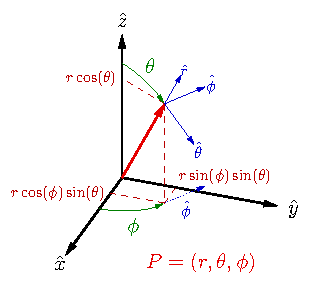
\includegraphics[width=0.42\textwidth]{pictures/spherical_coordinates.pdf}}%
    \hspace*{0.08\textwidth}%
    \subfloat[Cylindrical Coordinates]{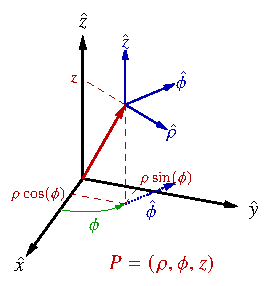
\includegraphics[width=0.38\textwidth]{pictures/cylindrical_coordinates.pdf}}

    \caption{Examples of curvilinear coordinates}
    \label{fig:spherical_cylindrical_coords}
\end{figure}



        \subsection{Areas \& Volumes in Curvilinear Coordinates}

volume element is $dV = dx \, dy \, dz$, with transformation into curvilinear coordinates applied; but we do not want to calculate this explicitly, too nasty, so we look at plot instead (Fig.~\ref{fig:spherical_coords_are_vol_el} (b)). volume element has thickness $dr$ in radial direction; in polar direction we cut out a piece of length $d\theta$ from a circle with circumference $r$; in azimuthal direction, we cut out a piece of length $d\phi$ from a circle of radius $r \sin(\theta)$ (different radius compared to polar direction is easily explained, for polar we rotate the whole vector basically, but for azimuthal we must keep the $z$-component fixed; and just like we can find radius of polar circle by noticing that it goes through $z$-axis $\equiv (0, 0, r)$, we find radius of azimuthal circle by noticing it goes through $x$-axis $\equiv (r \sin(\theta), 0, 0)$, or equivalently through $y$-axis $\equiv (0, r \sin(\theta), 0)$); forming the product of these three yields the correct result,
\begin{equation}
    \eqbox{
        dV = dr \, r d\theta \, r \sin(\theta) d\phi = r^2 \sin(\theta) \, dr \, d\theta \, d\phi
    }
\end{equation}


-> better justification for this: now, say we start at some position $\vec{r}$ and then go a step $dx$, then $dy$, then $dz$; this will form shape that can be completed to a cube basically and volume of this (infinitesimal) cube is $dV = dx \, dy \, dz$; but if we go $dr$, then $d\theta$, then $d\phi$, what we end up with is a shape that does \emph{not} have volume $dV = dr \, d\theta \, d\phi$; from plot, this makes sense, because length that we move when making step $d\phi$ for example from some position $\vec{r}$ actually depends on the position now; this is an effect of being in curvilinear coordinates and we have to use correction factor to account for this in $dV$ (this factor is called Jacobi determinant); more explicitly, this is idea: $(r, \theta, \phi + d\phi) - (r, \theta, \phi) \neq (0, 0, d\phi)$ \todo{verify this is actually true and related to Jacobi; should be, though -> ah, maybe idea is $x(r, \theta, \phi + d\phi) - x(r, \theta, \phi)$ is dependent on point and does not reduce to constant multiplied by $d\phi$ (?)}, an infinitesimal step works different in these types of coordinates; basically, when I make step $d\phi$ from $\vec{r}$, then the actual step I make (= length of step in Cartesian) is $r \sin(\theta) d\phi$
% $(r + dr, \theta + d\theta, \phi + d\phi) - (r, \theta, \phi) \neq (dr, d\theta, d\phi)$ -> overkill here, since all couple with each other, right?
-> just say: we plot $(r, \theta, \phi)$ and $(r, \theta, \phi + d\phi$); expectation: angular step we have to make to connect them is simply $d\phi$; but this is not true, actually we have to make $r \sin(\theta) d\phi$ -> maybe "angular step" is wrong word here (I refer to arclength of circle that connects them; this is path following $\vec{e}_\phi$ between the two points, i.e.~how we would compute the distance in components basically), but idea is certainly true! And perhaps simplest way to explain, do not try to use differences of components here -> though $(r, \theta, \phi + d\phi) - (r, \theta, \phi) \neq (0, 0, d\phi)$ might actually be true, now that I see argument with $\vec{e}_\phi$ here, this is exactly what we say there, don't we?
-> key idea is really: in Cartesian, when drawing $(x,y,z)$ and $(x+dx,y+dy,z+dz)$, then their distance in each direction really is the corresponding infinitesimal step; but when I draw $(r, \theta, \phi)$ and $(r, \theta, \phi + d\phi)$, then the step I have to make is not than $d\phi$, but depends on point (obvious from plot, but non-trivial when we try to write this down as expression involving components; SO REALLY DO NOT TRY)



from this we get area element easily, just don't multiply with $dr$ (which can be seen as differentiation with respect to $dr$):
\begin{equation}
    \eqbox{
        dA = r d\theta \, r \sin(\theta) d\phi = r^2 \sin(\theta) \, d\theta \, d\phi
    }
\end{equation}



\begin{figure}
    \centering

    \subfloat[Area Element]{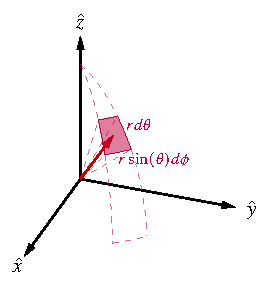
\includegraphics[width=0.44\textwidth]{pictures/spherical_coordinates_area_el.pdf}}%
    \hspace*{0.08\textwidth}%
    \subfloat[Volume Element]{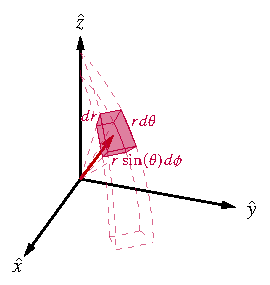
\includegraphics[width=0.36\textwidth]{pictures/spherical_coordinates_vol_el.pdf}}

    \caption{Area and volume element in spherical coordinates.}
    \label{fig:spherical_coords_are_vol_el}
\end{figure}



        \subsection{Polar Coordinates}


polar coordinates are just spherical coordinates (Eq.~\eqref{eq:spherical_coords}) with $\theta = 90\degree$ (and we get $dA$ from $dV$ by formally setting $d\theta = 1$) -> thus trick: remember spherical coordinates, then how they reduce

-> alternatively, cylindrical with $z = 1$


\begin{equation}\label{eq:polar_coords}
    \eqbox{
        \mqty(x \\ y) = \mqty(r \cos(\phi) \\ r \sin(\phi))
    }
\end{equation}



\begin{figure}
    \centering

    \subfloat[Definition]{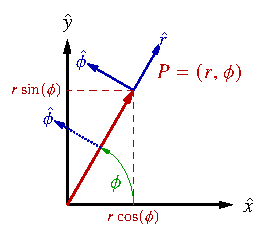
\includegraphics[width=0.4\textwidth]{pictures/polar_coordinates.pdf}}%
    \hspace*{0.08\textwidth}%
    \subfloat[Area Element]{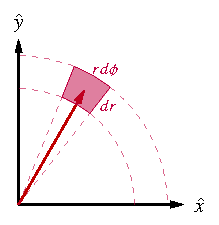
\includegraphics[width=0.4\textwidth]{pictures/polar_coordinates_area_el.pdf}}

    \caption{Polar Coordinates}
    \label{fig:polar_coordinates}
\end{figure}



    \section{Differential Geometry}

we take approach inspired by Thorne+Blandford: cite relatively advanced math, trading elegance and robustness of expressions for readibility if one is not familiar with some advanced calculus (mainly)


definition of gradient of a function: components of differential, i.e.
\begin{equation}
    \eqbox{
        df = \langle \grad f, d\vec{x} \rangle = \sum_i \pdv{f}{x^i} dx_i
    }
\end{equation}

-> this can be generalized to tensors of arbitrary rank by means of covariant derivative (cf.~Thorne+Blandford)



Stokes' theorem is all you need to know in order to remember how to connect differential conservation laws and corresponding integration laws (Gauß, Stokes, Green, fundamental theorem of calculus) -> cf.~1.8 of Thorne+Blandford

\begin{thm}[(Generalized) Stokes' Theorem]
    For orientable manifold $M$ with boundary $\partial M$
    \begin{equation}
        \eqbox{
            \int_M d\omega = \int_{\partial M} \omega
        }
    \end{equation}
\end{thm}




Hodge duality formalizes identification of are element $dA$ with normal vector of this are, e.g., $* dx = dy \wedge dz \equiv dA$ -> explains components of rotation, right? See H\_Analysis, page 203 (Beispiel 6.22)

-> for 1-form $g = g_\mu dx^\mu = \langle \vec{g}, d\vec{x} \rangle$, we have $dg = d \langle \vec{g}, d\vec{x} \rangle = \langle \curl \vec{g}, * d\vec{x} \rangle$. So demanding $g$ is conservative amounts to demanding the good-old condition of vanishing curl


rule to memorize laws: we need $n$-differential form to be able to integrate on $n$-dimensional manifold. So we need something with a single coefficient for this ($n$-form only has one; $n - 1$-form would have two coefficients etc), and curl as vectorial quantity would have three, so we need divergence as scalar quantity serving as single coefficient here


nice to memorize area integral: $\int_S \vec{v} \, d\vec{A} = \int v_x \, \hodge dx + \int v_y \, \hodge dy + \int v_z \hodge dz$ -> integrate components over area to which unit vector for this component is the normal vector (we get this area from normal vector using hodge star) \todo{check how components of normal vector enter here, there should be some kind of inner product with it involved...} -> we want flux of vector field through the surface, so we must extract component that flows through the surface, which is done via projection onto normal vector ($d\vec{S}$ is just notation); after that it is just surface integral of scalar function with area element $dS$


H\_Analysis, Beispiel 6.47

\begin{ex}[Gauß's Law/Theorem]
    $M = \mathbb{R}^3$ or rather subset thereof

    note that $dV$ and $d^3x$ are the same
\end{ex}


\begin{ex}[Stokes' Theorem]
    $M = \mathbb{R}^2$ or rather subset thereof
\end{ex}


\begin{ex}[Fundamental Theorem of Calculus]
    $M = \mathbb{R}$ or subset thereof
\end{ex}


\begin{ex}[Green's Law/Theorem]
    hmmm what is $M$ here?
\end{ex}


-> using $\oint$ instead of $\int$ indicates that we assume closed curve/surface




another important law is Gauß's law (\emph{another} Gauß law...):
\begin{equation}
    \eqbox{
        \delta(\vec{r} - \vec{r}_0) = \frac{-1}{4 \pi} \nabla^2 \frac{1}{\norm{\vec{r} - \vec{r}_0}}
    }
\end{equation}




    \section{Calculus Of Variations}

displacements are considered instantaneous, meaning
\begin{equation}
    \eqbox{
        \delta t = 0
    }
\end{equation}
Moreover (Thornton+Marion, Eq.(7.132)),
\begin{equation}
    \eqbox{
        \delta \dot{x}_i = \delta \dv{x_i}{t} = \dv{t} \delta x_i = 0
    }
\end{equation}


any variation $\delta$ is usually expressed in terms of a derivative $\pdv{\alpha}$; therefore, it is not surprising that we have something like a chain rule for it:
\begin{equation}
    \eqbox{
        \delta H(q_i, p_i) = \sum_i \pdv{L}{q_i} \delta q_i + \pdv{H}{p_i} \delta p_i
    }
\end{equation}



difference to derivative: variation is applied to a function of functions (a functional), i.e.~the result is not a point (the way it is for derivative), but rather a whole function

-> i.e.~for $J = J[f(x), g(x)]$,
\begin{equation}
    \eqbox{
        \delta J \coloneqq \eval{\dv{\epsilon} J'[f(x), g(x)]}_{\epsilon = 0} = \eval{\dv{\epsilon} J[f(x) + \epsilon h(x), g(x) + \epsilon h'(x)]}_{\epsilon = 0}
    }
\end{equation}

-> I guess in modern mathematics, we can argue that a function is also just a point in a space (?)


\end{document}